\documentclass[fontsize=12pt, paper=a4, headinclude, twoside=false, parskip=half+, pagesize=auto, numbers=noenddot, open=right, toc=listof, toc=bibliography]{scrreprt}

%\usepackage[inner=4cm,outer=2cm]{geometry}
%\setlength{\oddsidemargin}{15,5pt}
%\setlength{\evensidemargin}{15,5pt}


%parskip:
  % full - Absätze haben großen Abstand
  % half - Absätze haben kleinen Abstand
  % off - Absätze haben Einzug (default)

% Bessere Unterstützung für PDF-Features
\usepackage[breaklinks=true]{hyperref}

%Schönere Schriftart laden
%\usepackage[latin1]{inputenc}
\usepackage[T1]{fontenc} % Ligaturen, richtige Umlaute im PDF
\usepackage[utf8]{inputenc}% UTF8-Kodierung für Umlaute usw
\usepackage[english]{babel} % Deutsche Silbentrennung verwenden
\usepackage{lmodern}
\renewcommand*\familydefault{\sfdefault}  %Zusatz für serifenlose Schrift.

%Zeilenabstand
\usepackage{setspace} % Zeilenabstand
\onehalfspacing % 1,5 Zeilen

% Schriften-Größen
\setkomafont{chapter}{\Huge\rmfamily} % Überschrift der Ebene
\setkomafont{section}{\Large\rmfamily}
\setkomafont{subsection}{\large\rmfamily}
\setkomafont{subsubsection}{\large\rmfamily}
\setkomafont{chapterentry}{\large\rmfamily} % Überschrift der Ebene in Inhaltsverzeichnis
\setkomafont{descriptionlabel}{\bfseries\rmfamily} % für description Umgebungen
\setkomafont{captionlabel}{\small\bfseries}
\setkomafont{caption}{\small}



% Einfachere Verwendung von korrekten Anführungszeichen
\usepackage[german=guillemets]{csquotes}
% oder german=quotes
% oder english=british oder english=american

%Mathematisches
\usepackage{amssymb}
\usepackage{amsmath}
\usepackage{amsthm}

%Quelltext einbinden
\usepackage{algorithm}
\usepackage{algorithmic}

%Abbildungen
\usepackage{graphicx}
\usepackage{caption}
\usepackage{subcaption}
\usepackage[verbose]{wrapfig}
\usepackage{float}
%\restylefloat{figure} %kannst du einen weiteren Positionierungsparameter [H] definieren. der setzt dir das bild an genau die stelle, wo du es haben willst. Ist allerdings auch nicht immer so praktisch.
% wenn du ein \pagebreak einfügst, gibt er dir vor der neuen seite noch alle gleitobjekte aus, die noch anstehen

%Zeichnen mit Tikz
\usepackage{tikz}
\usetikzlibrary{intersections,positioning,shapes.geometric,calc}

% Tabellen
\usepackage{multirow} % Tabellen-Zellen über mehrere Zeilen
\usepackage{multicol} % mehre Spalten auf eine Seite
\usepackage{tabularx} % Für Tabellen mit vorgegeben Größen
\usepackage{longtable} % Tabellen über mehrere Seiten
\usepackage{array}

%Bibliographie
\usepackage[square, comma, numbers, sort&compress, round]{natbib}
\usepackage{bibgerm} % Umlaute in BibTeX

%Umbenennung der vordefinierten definition- und example-Umgebung
\theoremstyle{definition}
\newtheorem{lecture}{Lecture}
\newtheorem{definition}{Definition}
\newtheorem{example}{Example}
\newtheorem{lemma}{Lemma}

% \newtheorem{theorem}{Satz}
% \newtheorem{constructing instructions}{Konstruktionsvorschrift}
% \newtheorem{properties}{Eigenschaften}
%\newtheorem{proposition}{Proposition}
%\newtheorem{korollar}{Corollary}
%\newtheorem{remark}{Remark}
%\newtheorem{consequences}{Consequences}
%\newtheorem{observation}{Observation}
%\newtheorem{conjecture}{Conjecture}
%\newtheorem{recall}{Recall}

\renewcommand{\labelenumi}{\roman{enumi})}

\renewcommand{\labelitemii}{$\bullet$}

\newcommand{\todo}[1]{
      {\colorbox{red}{ TODO: #1 }}
}
\newcommand{\todotext}[1]{
      {\color{red} TODO: #1} \normalfont
}

%bzgl `tocbasic` Warnung
\usepackage{scrhack}
 % Importiere die Einstellungen aus der Präambel
% hier beginnt der eigentliche Inhalt

\author{Lydia Buntrock}
\title{master thesis}
\date{Januar 2018}

\hfuzz=\maxdimen \tolerance=10000 \hbadness=10000
% \usepackage[showframe=true]{geometry}


\begin{document}
  % Titelseite
  \begin{titlepage}
    \pagestyle{empty}
  	
    	\vspace{20mm}
    	\begin{Large}
          \textbf{An analysis of maximum parsimony algorithms to predict parasitism in Eukaryota}\\
          using a large multiurcated phylogenetic synthesis tree
      \end{Large}

  	\clearpage
  \end{titlepage}

%---------------------------------------------------------------------------------------------------
%---------------------------------------------------------------------------------------------------
%---------------------------------------------------------------------------------------------------
%--------------------------------------------------------------------------------------------------- 
\chapter*{Abstract}
  With increasing amounts of data, new investigations are also possible in phylogeny. This study 
    deals with the ancestral state reconstruction of parasitism in the tree of life of eukaryotes. 
    We predict unknown states of species and estimate origins and losses of parasitism. \\
  We performed an analysis of existing algorithms and selected a Sankoff maximum parsimony algorithm 
    using the R package \textit{Castor} \cite{Louca2017}. \\
  The challenge here is the size of the tree and the little information about it. \\
  Such a large phylogenetic tree does not completely exist and therefore we work with a synthesis 
    tree of OTL \cite{Hinchliff2015} which is highly multifurcated. \\
  For the 2,535,437 leaf nodes we could not gather much data. From the GloBI database 
    \cite{Poelen2014} whith we used for this, we could only collect 25,992 parasitic and 34,879 
    free-living species. It follows that we have only $\approx 2.4\%$ state information. \\

  Nevertheless, the analysis of our results revealed that our forecast is largely credible. \\
  We have compared the results of some subtrees with known knowledge (Chordata, Nematoda, 
    Platyhelminthes and Apicomplexa) and except for the Nematoda the results looked very good. In 
    the case of nematodes, the data situation is strongly shifted to the few parasites. \\
  Our number of origins we could partly compare with the results of Sara B. Weinstein and Armand M. 
  Kuris from their article \textit{Independent origins of parasitism in Animalia} \cite{Weinstein2016} 
    and have come to a similar magnitude. They identified 223 parasitic origins in Metazoa and we 
    were able to estimate about 300 origins. \\

    
\tableofcontents
\clearpage

%---------------------------------------------------------------------------------------------------
%---------------------------------------------------------------------------------------------------
%---------------------------------------------------------------------------------------------------
%--------------------------------------------------------------------------------------------------- 
\chapter{Introduction}
  This paper is about the further development of parsimony algorithms for non-binary trees, applied 
  to the currently largest phylogeny synthesis tree of Open Tree Of Life, with the application to 
  the ancestral state reconstruction of parasitism. \\
  \anmerkungstext{Der erste Satz muss nochmal überarbeitet werden. Das Ziel / Ergebnis der Arbeit 
    hat sich inzwischen geändert} \\
  \anmerkungstext{Wir haben mehr einen Algorithmus getestet und an unserem spezifischen Problem angewendet, 
    als viel selbst zu entwickeln. Allerdings haben wir den Fitch Algorithmus von binär auf multinär 
    umgeschrieben.} \\

  \anmerkung{Mein Vorschlag einer Gliederung (jeweils ca. ein Absatz) (Bernhard)}
  \begin{enumerate}
    \item Motivation:
      \begin{itemize}
        \item Was ist das große Ziel? \\
          Das Ziel dieser Arbeit ist die Anwendung von maximum parsiomony algorithmen auf nicht 
          binäre Bäume und auf sehr große Datensätze. Insbesondere auf das Beispiel 'Entstehung des 
          Parasitismus' im ganzen Eukaryotischen Tree of Life.
        \item Was soll erreicht werden? \\
          Wir wollen vorhandene Algorithm (Sankoff/castor \cite{Louca2017}) auf diese Aufgabenstellung hin testen 
          und ihre Vorhersagekraft abschätzen. Außerdem wollen wir den Fitch algorithmus für binäre 
          Bäume auf unser Problem erweitern und mit dem Sankoff Algorithmus vergleichen.
        \item Warum ist das relevant? Was könnte man dann tun?\\
          predict states of species... \\
          \todo{!!!}
      \end{itemize}
    \item Hintergrund:
      \begin{itemize}
        \item Was gab es in dieser Richtung bereits als ganze Ansätze oder wenn nicht, warum nicht?
          Woran ist es bisher gescheitert? \\
          Bisher wurden vorallem Algorithmen für das binäre Problem entwickelt, da man wesentlich 
            kleinere Teilbäume betrachtet hat, von welchen man auch alle Aufspaltungen kennt. Durch 
            die Entwicklung von OTL, eines gesamten Baum des Lebens, ergibt sich das Problem, dass 
            dieser bei weitem nicht binär ist. \\ \\
  Researchers of the phylogenies have been dealt with the ancenstral state reconstruction in the 
    60s. The first methods were only brute force \todo{Quelle, siehe Fitch: Camin and Sokal 1965}. 
    Next came a set of parsimony algorithms such as: Fitch-parsimony \cite{Fitch1971}, 
    Wagner-parsimony \cite{Swofford1987} ... \todo{weitere?}. \\
    With more and more data, there is now the possibility to use more information to calculate the 
    probabilities of the ancestral states. In addition to the states of the leafs, algorithms could 
    also use branch lengths. The likelihood based algorithms came more in interest. \\
    Our focus came with another 'data extension'. We wanted to work with the biggest phylogenetic tree 
    that exists at this moment, which goes over all observed species. For most \todo{most?} species 
    there is no phylogeny, but only a taxonomic classification.
  
        \item Welche Grundlagen sind notwendig:
          \begin{itemize}
            \item open tree of life: Was ist das, warum relevant und überlegen als reine Ansätze? \\
              \todo{!!!} \\ \\
  So the biggest 'phylogenetic tree' is a synthesis 
    of phylogenetic trees filled with a taxonomic tree given by Open Tree of Life \cite{Hinchliff2015}.
    This tree is not binary and therefore the developed algorithms are not directly applicable. \\
            \item Algorithmen: Was gibt es? Ruhig ausführlicher als hier bereits und vor allem auch 
              nach einer Darstellung am Ende ableiten, was für uns relevant ist. Also beschreiben, 
              wie Methode a, b, c funktionieren und dann abwägen, was daher für Dich am 
              relevantesten ist. \\
              \todo{!!!} \\
              \anmerkung{GloBI und OTL in der Einleitung vorstellen. (Emanuel)}
          \end{itemize}
      \end{itemize}
    \item Outlook/Structure of this work
  \end{enumerate}


  In this work, we have looked at the algorithms that are generally suited to our data, to develop 
  them further for the not binary case, and finally to compare their usability with our sythesis 
  tree. \\
  We have decided to consider only parsimony algorithms since we have no information on branch 
  lengths and no other additional information like different transition probabilities of our states.

  %---------------------------------------------------------------------------------------------------
  %---------------------------------------------------------------------------------------------------
  %--------------------------------------------------------------------------------------------------- 
  \section{Definitions}
    \begin{itemize}
      \item Parasit - Freilebend
      \item Multifurkation - binär
      \item height (min, max, mean), depth of a tree/node (Distanz zur Wurzel vs distanz zum Blatt)
      \item maximum parsimony
      \item OTL, OTT, GloBI
    \end{itemize}

%---------------------------------------------------------------------------------------------------
%---------------------------------------------------------------------------------------------------
%---------------------------------------------------------------------------------------------------
%--------------------------------------------------------------------------------------------------- 
\chapter{Methods}
  As initiated, we would like to apply a maximum parsimony algorithm to the entire tree of life to 
    obtain an ancestral state reconstruction of free-living versus parasite states. \\
  So far, these reconstructions have been made mainly on binary trees with better data availability. 
    Therefore, we decided to use a simulation to decide how to evaluate the existing algorithms and 
    possibly adapt them to our given problem. \\
  Accordingly, in addition to the necessary data sets (GloBI, OTL), the chosen algorithm and the 
    evaluation of its results, this chapter also deals with the previously performed simulation and 
    the evaluation of the various algorithms and their parameters. \\
  Figure \ref{fig:workflow} briefly outlines these relationships.
  \begin{figure}[h!]
    \centering
    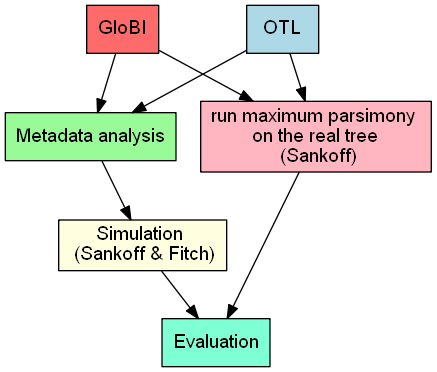
\includegraphics[width=0.4\textwidth]{Figures/Workflow-overview.png}
    \caption{Workflow \\
      The coming sections are thus subdivided into the following topics: \\
      \todo{or:} The resulting procedure is as follows: \\
      (1) Get the real tree and real data for the leaf nodes $\rightarrow$ OTL, GloBI databases.
      (2) Get metadata of these for a realisitc the simulation.
      (3) Build and run the simulation.
      (4) Evaluation of parameters for the simulation and the real problem.
      (5) Run the resulted algorithm on the original data.
      (6) Evalute and interprete results. $\rightarrow$ Origins etc...
    }
    \label{fig:workflow}
  \end{figure} \\
  \todo{Metadata analysis nötig für run maximum parsimony?} \\

  % \begin{enumerate}
  %   \item Get the real tree and real data for the leaf nodes. $\rightarrow$ OTL, GloBI databases
  %   \item Get metadata of these for a realisitc the simulation.
  %   \item Build and run the simulation.
  %   \item Evaluation of parameters for the simulation and the real problem.
  %   \item Run the resulted algorithm on the original data.
  %   \item Evalute and interprete results. $\rightarrow$ Origins etc...
  % \end{enumerate}
  
  \begin{figure}[h!]
    \caption{Workflow}
    \centering
    \label{fig:Workflow}
    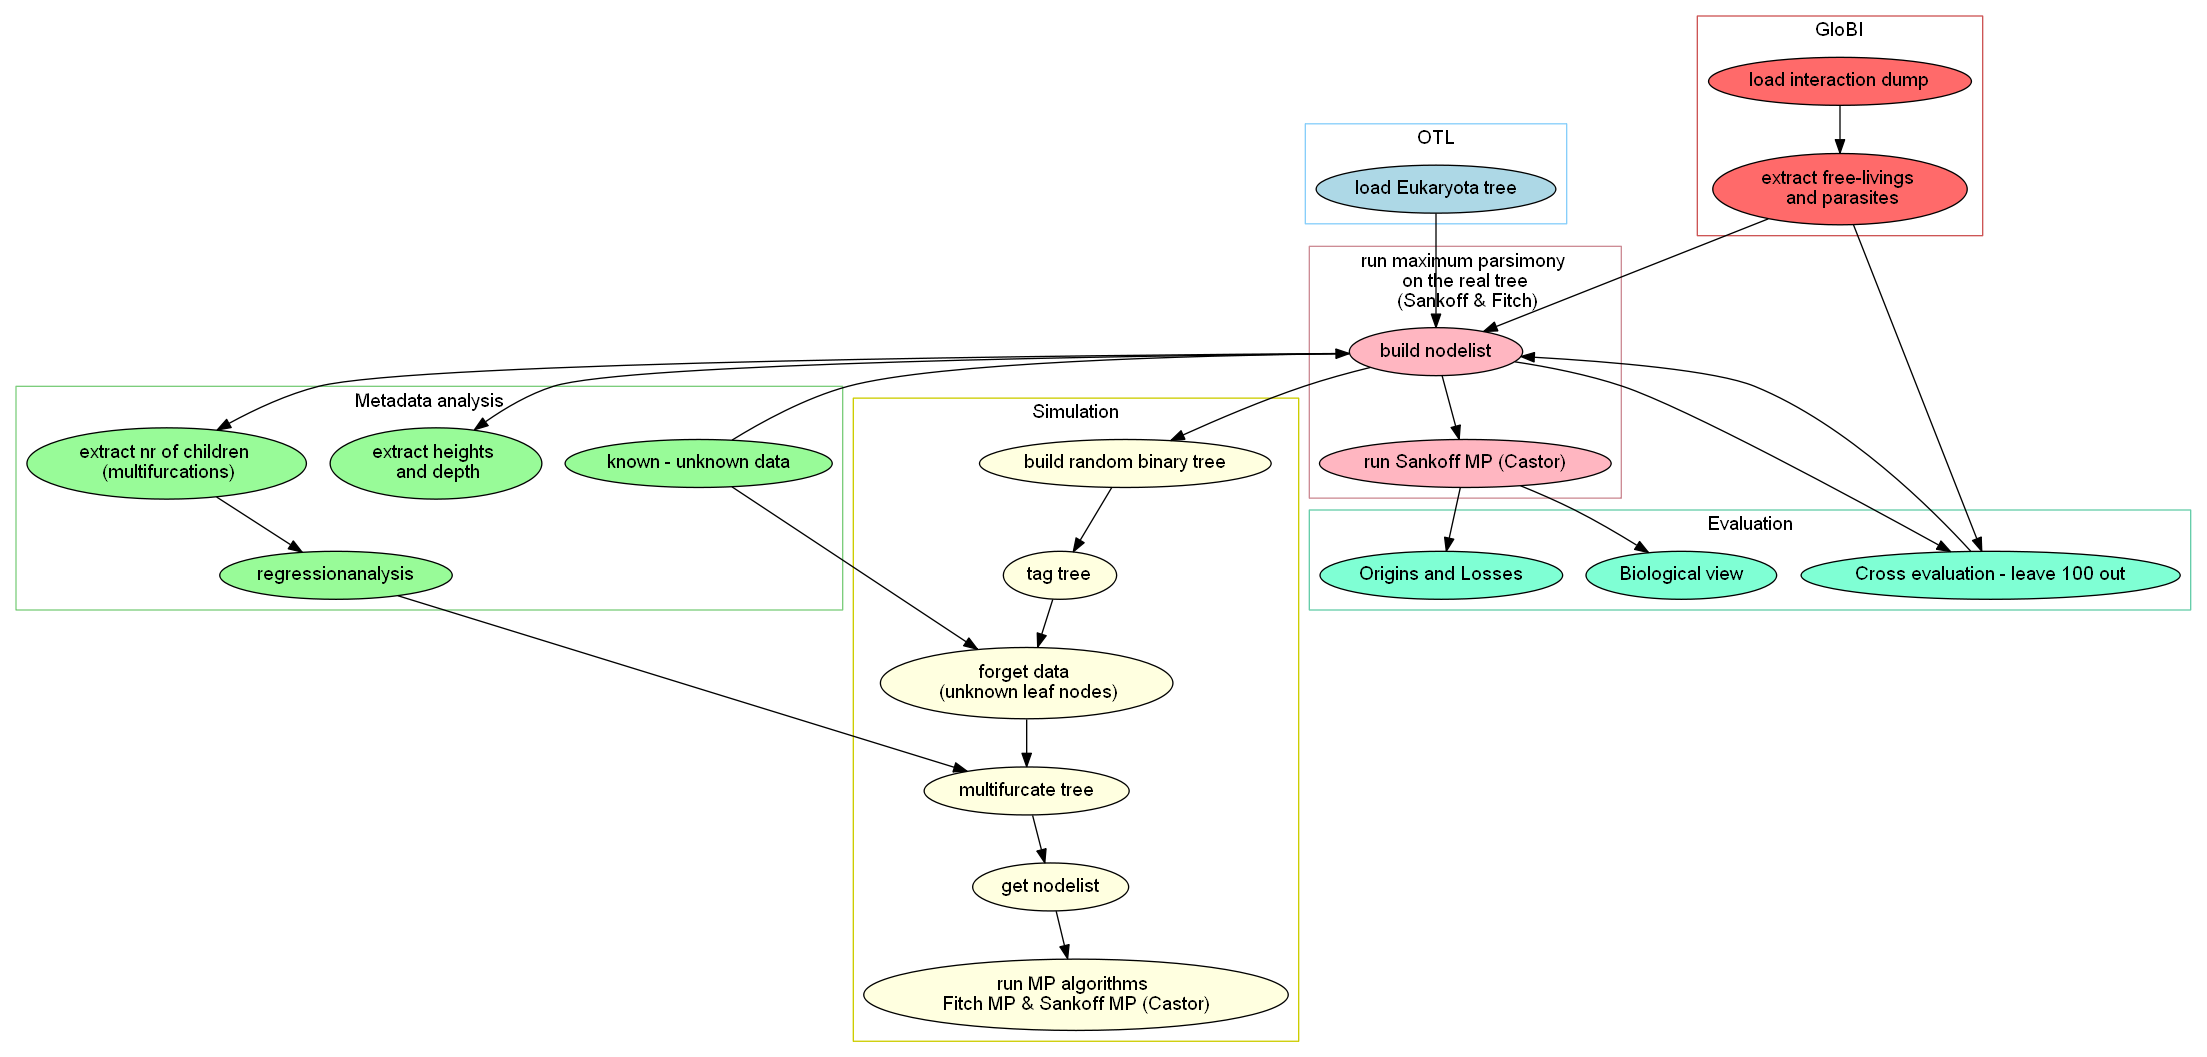
\includegraphics[width=1\textwidth]{Figures/Workflow.png}
  \end{figure}

  %---------------------------------------------------------------------------------------------------
  %---------------------------------------------------------------------------------------------------
  %---------------------------------------------------------------------------------------------------
  \section{Get data - Properties of real Data}
    For our research we need two types of data: a tree and information about the states. \\
    For the tree we decided to use Open Tree of Life (OTL), because it's the biggest available synthesis 
      tree. \\
    \todo{hier referenzen zu nem paper das das bestätigt o.ä.} \\
    For the state information, we decided to use the Global biotic interaction database (GloBI). Also in 
      this case, this is one of the largest databases and both OTL and GloBI support the OTT 
      identification. OTT (open tree taxonomy) is a taxonomy that assigns to each species a unique id, 
      both ancestor and now living species (internal and leaf nodes).

    %---------------------------------------------------------------------------------------------------
    %---------------------------------------------------------------------------------------------------
    \subsection{OTL}
      For our project we looked for a large database for phylogenetic trees and also for a taxonomic 
        tree. Since we run our algorithm on the phylogenetic tree, and for the evaluation and other 
        properties the taxonomy provides us with much more information. \\
      OTL gives us both. A synthesis of phylogenetic trees (currently 819 trees) and a taxonomic tree. 
        OTL also includes the large phylogenetic database TreeBASE \cite{Hinchliff2015}. \\
      \todo{Das steht auf der Website nicht in dem Paper...} \\
      For phylogenetic data, there are at least five big data collections, namely: ITIS (Integrated 
        Taxonomic Information System) \cite{ITIS}, NCBI (National Center for Biotechnology Information) 
        \cite{NCBI1988}, WORMS (World Register of Marine Species) \cite{WoRMS2018}, GBIF (Global 
        Biodiversity Information Facility) \cite{GBIF}, OTT (OpenTreeOfLife-Taxonomy) 
        \cite{Hinchliff2015}. \\
      \todotext{Marius:} "Every dataset has it's own characteristics and downsides. ITIS is only a small 
        set of 100\% confirmed and named species. GBIF is not composed with the help of phylogeny, the 
        same is valid for the NCBI taxonomy. The WORMS taxonomy is a way too small dataset of mostly 
        marine species. \\
      We choosed the taxonomy from OpenTreeOfLife because it's including most of the known taxonomies 
        and got synthesised by preffering taxonomies that match with available phylogenetic data. At the 
        same time the team from OTL preferred a maximum number of species \cite{Hinchliff2015}. This is 
        resulting in somekind of hybrid between taxonomy and phylogeny." \\

      %---------------------------------------------------------------------------------------------------
      \subsubsection{Distribution of Taxa}
        - In our tree we can distinguish 28 different Taxa with the OTL taxonomic tree. \\
        - The most of them are hardly represented. The major taxonomic groups are: ... \\
        - Here you can see some characteristics of the Multifurcation of the tree. \\
        \begin{figure}[h!]
          \centering
          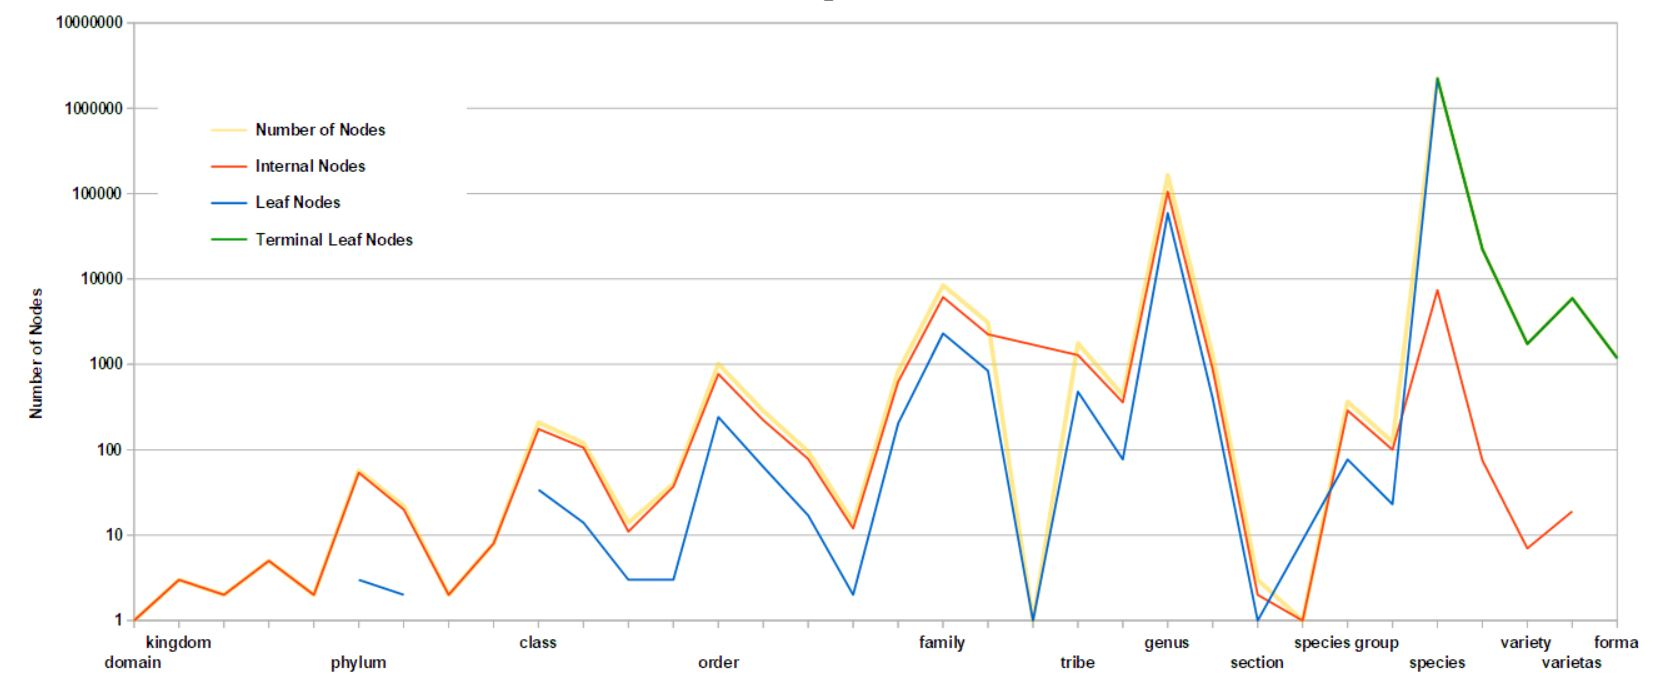
\includegraphics[width=0.9\textwidth]{Figures/TaxaTable2.JPG}
          \caption{Distribution of Nodes in Rank-Cathegories}
          \label{fig:taxaTable2}
        \end{figure}
        In a phylogeny, the taxonomic division of the tree is far too coarse, meaning that there should 
          be more subtaxa or 'unranked' nodes. But the closer we get to the root, the more the pure
          taxonomic tree is reflected. If the tree were binary, the taxa would have to double. But the 
          multipliers for some are much bigger and for others much smaller, which you can see in in figure 
          \ref{fig:taxaTable2}. \\
        Please see the appendix on page \pageref{sec:taxaTable2} for a complete table \ref{sec:taxaTable2} 
          of these data. \\
        \todo{Was hierzu ist richtig und wichtig?}

      %---------------------------------------------------------------------------------------------------
      \subsubsection{Distribution of data in the taxa}
        Mithilfe des taxonomischen Baums von OTL haben wir die Knoten ihren Kingdoms, Phyla und Classes 
          zugeteilt. \\
        Please see the appendix on page \pageref{sec:taxaTable1} for a complete table \ref{sec:taxaTable1} 
          of these data. \\
        \todo{gibt es einen Zusammenhang zwischen Anzahl} \\
        \todo{max max height zu anzahl nodes in phylum plotten? oder mean max height oder ... 
          (mean, min height...)} \\
        \todo{depth...}

    %---------------------------------------------------------------------------------------------------
    %---------------------------------------------------------------------------------------------------
    \subsection{GloBI}
      \todotext{Marius:} "There aren't many big active interaction databases out there, most of them are 
        offline or outdated. For example: IWDB (Interaction Web Database) \cite{IWDB2003}, Webs on the 
        Web \cite{WOW2004}, Animal Diversity Web \cite{Myers2003} and ecoweb \cite{Cohen2010}. GloBI is 
        including most of the known ones and is still growing actively \cite{Poelen2014}. So the 
        question which interaction database could be used was answered rather quickly." \\

      This database consists of entries of the form: species A (source) interacts with B (target). \\
      We appointed some interactions, where we know from the biological perspective that the species 
      source or target has to be a parasite or a free-living species. These are the following:
      \begin{itemize}
        \item free-living source: preysOn, eats, flowersVisitedBy, hasPathogen, pollinatedBy, 
          hasParasite, hostOf
        \item free-living target: preyedUponBy, parasiteOf, visitsFlowersOf, pathogenOf, hasHost
        \item parasite source: parasiteOf, pathogenOf
        \item parasite target: hasParasite, hasPathogen
      \end{itemize}
      \todo{Interactions nochmal prüfen! Darauf basieren unsere Ergebnisse!} \\
      We build two lists: parasites and free-livings, and add the source or targets of an interaction
        to these. \\
      \todo{klar? Oder Beispiel bringen? (Katze isst Maus $\rightarrow$ Katze ist Freilebend)} \\
      % For every interaction from these lists, we get one or two species for our parasite or 
      %   free-living lists.
      \todo{einige spezies nicht mit einbezogen, da sie keine OTT id haben, hier könnte man noch 
        verbessern (future work)}
      \todo{You can find all interaction types here:
        https://github.com/jhpoelen/eol-globi-data/blob/master/eol-globi-lib/src/main/java/org/eol/globi/domain/InteractType.java .} \\ \\
      
      With this we got $\sim 51000$ (distinct) freeliving species and $\sim 47000$ (distinct) parasite 
        species (see section countings) \todo{ref einfügen}. But we found also  $\sim 57000$ (not 
        distinct) source species and $\sim 810000$ (not distinct) target species without OTT ids. 
        Since we currently use only OTT ids, we could not use this information. \\
      \todo{mehr dazu in section: unknown nodes...}

  %---------------------------------------------------------------------------------------------------
  %---------------------------------------------------------------------------------------------------
  %---------------------------------------------------------------------------------------------------
  \section{Metadata analysis}
    Um eine möglichst realistische Simulation zu erzeugen haben wir auf der einen Seite einige Daten 
      gesammelt (vorheriges Kaptiel), und außerdem beeinflussende Parameter untersucht. \\
    Wir haben zwei große Arten von Parametern:
    \begin{enumerate}
      \item Biological parameters (A result of the evolutionary process.):
        \begin{itemize}
          \item transition probabilities
        \end{itemize}
      \item Distribution of the loss of information:
        \begin{itemize}
          \item Loss of topology ($\rightarrow$ mutlifurcations).
          \item Unknown information about the states of some leaf nodes.
        \end{itemize}
    \end{enumerate}
    We tested the influence of these parameters on our result using our simulation (Section 
      \ref{sec:simulation}).
   
    %---------------------------------------------------------------------------------------------------
    %---------------------------------------------------------------------------------------------------
    \subsection{Transition probabilities}
      \anmerkungstext{Wir hätten aber maximal 2 beta-Verteilungen mit jeweils 2 Parametern und je einem 
      eigenen Schwellenwert bei dem in die andere Verteilung gewechselt wird. Also 6 Parameter. Ich 
      finde den Parameterraum den du bisher betrachtest zum einen nicht systematisch erfasst, zum 
      anderen wahrscheinlich auch zu klein. Du kannst -Parameter sparen- indem zu z.B die beiden 
      Verteilungen und cut-offs symmetrisch (gespiegelt an 0.5) machst. Solltest aber meines Erachtens 
      die Schwellenwerte freier variieren. Das können wir bis zu unserem nächsten Treffen zurückstellen 
      und dann gemeinsam diskutieren. (Emanuel)} \\
      Das mit dem symmetrisch spiegeln geht halt nur bei maximal 40-60 Verteilungen richtig gut, danach 
      haben brauchen eventuell eine lange Austestphase, bis ein Baum dieser Verteilung entspricht.
      Wenn wir allerdings dafür zwei verschiedene Schwellenwerte einführen könnte das dieses Problem 
      eventuell ausgleichen. Das müsste ich austesten. 

      \todo{Kapitel tag tree hier einbinden}

    %---------------------------------------------------------------------------------------------------
    %---------------------------------------------------------------------------------------------------
    \subsection{Multifurcation}
      We have a very high multifurcation rate \pageref{sec:ResultsMultifurcation}.

      Therefore, the impact of multifurcations on our research question has been investigated:
      \begin{itemize}
        \item stärke der Multifurcation in verschiedenen Subbäumen
        \item zusammenhang zur tiefe im Baum
        \item zusammenhang zu höhe im baum (max, min, mean)
        \item einfluss auf die vorhersage des Castor und Fitch Algorithmus (Simulation) \todo{...}
      \end{itemize}

      "Nested models were compared using likelihood ratio tests, models using different predictors were 
      compared according to their deviance and AIC."
      \begin{lstlisting}[gobble=8]
        glm(formula = multifurc ~ 1, family = "poisson", data = inner.taxa)
      \end{lstlisting}

        % \todo{old Stuff:} \\
        %   Then we tried to find a function which best discribes this behavior. In figure 
        %   \ref{fig:HistogramsOfMultifurcations} is this plot shown with three functions, which came 
        %   closest to this goal: $\frac{1000000000000000}{x^4}$ (magenta), 
        %   $\frac{300000000000}{x^3}$ (red) and $\frac{80000000}{x^2}$ (black). \\
        % \begin{figure}[h]
        %   \caption{Histogram of multifurcations and fitting functions}
        %   \centering
        %   \label{fig:HistogramsOfMultifurcations}
        %   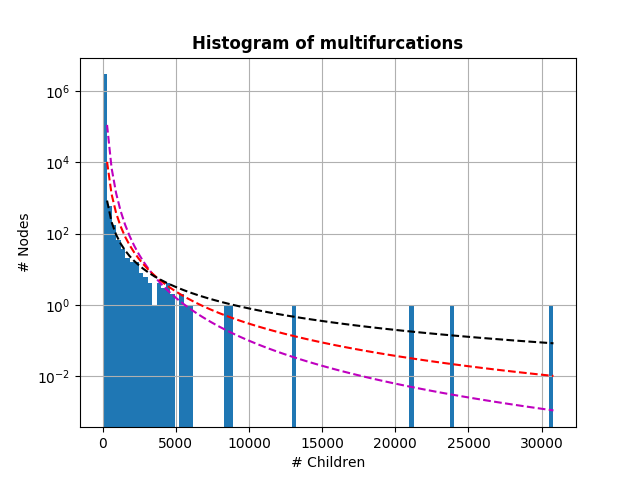
\includegraphics[width=0.7\textwidth]{Figures/HistogramsOfMultifurcations.png}
        % \end{figure}
        % From the biology we know, that this multifurcation is very clouded. Some parts of the tree are 
        %   well known and others have not been very interesting for the research so far. So we also wanted 
        %   to know how the multifurcations behave in some interesting subtrees. \\
        % \anmerkung{do we? Is that really universal knowledge or could it be supported by data or a citation? (Bernhard)} \\

  %---------------------------------------------------------------------------------------------------
  %---------------------------------------------------------------------------------------------------
  %---------------------------------------------------------------------------------------------------
  \section{Simulation}\label{sec:simulation}
    \anmerkung{Motivate the goal of the simulation (Bernhard)}
    \begin{itemize}
      \item build random binary trees, tag these (parameters: parasites vs free-living, 
        beta-distribution)
      \item run fitch-parsimony, wagner-parsimony, our parsimony like algorithm
      \item build not binary tree (poisson distribution?)
      \item run new algorithms
      \item compare trees (distances)
    \end{itemize}

    \begin{enumerate}
      \item build random binary trees
      \item tag tree
      \item multifurcate tree
      \item run maximum parsimony algorithms
      \begin{itemize}
        \item Fitch
        \item Sankoff (Castor package \cite{Louca2017}) 
        \item my algorithm
      \end{itemize}
      \item Evaluation
    \end{enumerate}

    %---------------------------------------------------------------------------------------------------
    %---------------------------------------------------------------------------------------------------
    \subsection{random binary tree}
      \anmerkung{Again, motivate first, why this is required and why you choose this solution (Bernhard)} \\
      To get a random binary tree, I used the Phylo package from biopython. They offer a randomized
        function which returns a BaseTree \footnote{
          https://github.com/biopython/biopython/blob/master/Bio/Phylo/BaseTree.py
        }:
      \begin{lstlisting}[gobble=6]
        from Bio import Phylo
        Phylo.BaseTree.Tree.randomized(number_leaf nodes)
      \end{lstlisting}
      From the BaseTree class:
      \anmerkung{trivial, does not give real info (Emanuel)}
      \begin{lstlisting}[gobble=6]
        def randomized(cls, taxa, branch_length=1.0, 
              branch_stdev=None):
        """Create a randomized bifurcating tree given a list
              of taxa.
          :param taxa: Either an integer specifying the number
              of taxa to create (automatically named taxon#), 
              or an iterable of taxon names, as strings.
          :returns: a tree of the same type as this class.
        """
      \end{lstlisting}
      \todo{Zitat von BaseTree und buildTree.py}

    %---------------------------------------------------------------------------------------------------
    %---------------------------------------------------------------------------------------------------
    \subsection{tag tree}
      \anmerkung{instead of 'tag tee' simulating states and transitions between them (Emanuel)} \\
      At this point we want one fully tagged tree, and one less tagged tree which looks like our real 
        data.\\
      Let's say the first specie (the root node) was free-living (start with a parasite without a host 
        makes no sence). For every transition from a node to his child, we take a random number from
        the father distribution. We decided that from the biological perspective a beta distribution
        reflects our transition probabilities best (see Figure 2.1 \todo{ref einfügen}). \\
      \anmerkung{why is that the case and why is that from a biological perspective? (Bernhard)} \\
      \anmerkungstext{I'd rather say that to ensure that the parameter of the binomial distribution is 
        restricted to the [0,1] interval, we model it... (Bernhard)} \\
      For example when our father node was free-living, then we take from the free-living beta
        distribution. Is the number under the threshold for beeing parasite, we get a change and tag
        the current node as parasite. Otherwise we tag it as free-living. \\
      With this procedure we traverse through the tree from the root to every leaf node. A part of
        this code you see here:
      \begin{lstlisting}[gobble=6]
        from numpy import random
        if father_tag == 0:
          # freeliving_distribution:
          new_random = random.beta(a=A_FL, b=B_FL)
        else:
          # parasite_distribution:
          new_random = random.beta(a=A_P, b=B_P)
        tag = 0         # $\rightarrow$ FL
        if new_random < percentage_parasites:
          tag = 1       # $\rightarrow$ P
      \end{lstlisting}
      \begin{figure}
        \caption{60\% Free-living - 40\% Parasites}
        \centering
          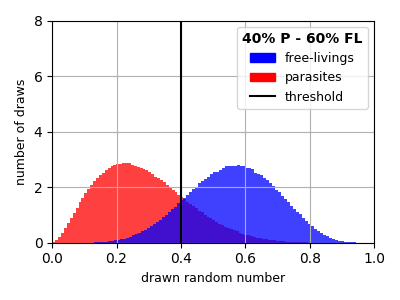
\includegraphics[width=0.5\textwidth]{Figures/40-60.png}
      \end{figure}
      \todo{Bessere Beschriftung, Plot neu erstellen! U.a. mit threshold} \\
      We save each tag with the associated node ID in a nodelist. \\
      \anmerkung{simulationg loss of information (1) states (2) topology/multifurcation (Emanuel)} \\
      The real tree has much less information, we have only information from some current species 
        (leaf nodes) and \todo{and probably negligible internal nodes}. \\
      To simulate our real tree we save for every node an empty placeholde except for some leaf nodes.
      There we save the states again. The amount of these unknown information is one parameter, which we
      got from our real tree. Or which we can change to \todo{...}
      \todo{Was hiervon gehört ind Methoden, was schon in Implementierung oder ganz woanders hin?}

    %---------------------------------------------------------------------------------------------------
    %---------------------------------------------------------------------------------------------------
    \subsection{multifurcate tree}
      \anmerkung{simulating loss of information (Emanuel)} \\
      Another parameter is the nature and strength of the multifunction of the tree, since we do not 
        have a binary tree in the real case. After several measurements and analyzes, which we explain 
        in \todo{section/chapter x}, \anmerkung{fit, justification (Emanuel)} we decided to use a $\frac{1}{x}$ distribution, where x is the depth 
        of a node. This means, how deaper we are, how less information we have. \\
      We traverse through the tree and pick a random number between 0 and 1. If random number is smaller 
        as our limit ($\frac{1}{x}$), than we forget the node and hang every child to the father node of 
        the current node. \\
      \anmerkung{poisson process $\rightarrow$ fit that distribution, include depth as a predictor, see if significant (Emanuel)}
      \begin{lstlisting}[gobble=6]
        from numpy import random
        from utilities import Helpers

        def get_non_binary_tree(subtree, nodelist):
          i = 0
          while i != len(subtree.clades):
            if subtree.clades[i].is_terminal():             # is leaf node?
              i += 1
            else:
              element = Helpers.find_element_in_nodelist(subtree.clades[i].name, nodelist)
              limit = get_limit(element[1])
              new_random = random.uniform()                 # choose if we want to delete ourselve
              if new_random < limit:                        # or new_random < 0.9:
                subtree.clades += subtree.clades[i].clades  # add children
                del subtree.clades[i]                       # delete internal node
              else:                                         # if we don't deleted ourselve go on with children
                get_non_binary_tree(subtree.clades[i], nodelist)  # otherwise the children are in the current clade array
                i += 1
          return

          def get_limit(depth):
            limit = 1 - 1 / ((depth + 3) / 4)
            if limit < 0.1:
              limit = 0.1
            return limit
      \end{lstlisting}
      % # current clades: clade_1 clade_2 ... clade_i-1 clade_i ... clade:_n
      % # add children of clade_i, delete clade_i
      % # new clades:clade_1 clade_2 ... clade_i-1 child_clade_1 ... child_clade_m ... clade:_n
      % # child_clade_1 is new clade i
      Wir lassen das Limit nicht beliebig klein werden, sondern beschränken es auf 0.1.

    %---------------------------------------------------------------------------------------------------
    %---------------------------------------------------------------------------------------------------
    \subsection{maximum parsimony algorithms}
      \subsubsection{Fitch maximum parsimony}
        Described from [COO98] + others ... - implemented for multifurcating trees

        Fitch algorithm for binary trees:
        \begin{figure}
          \caption{bla}
          \centering
            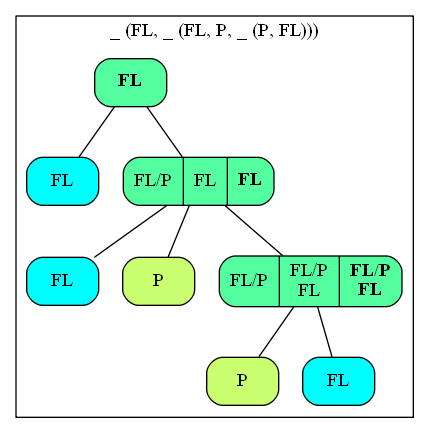
\includegraphics[width=0.5\textwidth]{Figures/Fitch1.png}
        \end{figure}

        Der Baum hat die folgende Struktur: Alle inneren Knoten sind leer. In den Blattknoten befindet 
        sich entweder das Tag FL oder P, oder deren Vereinigung, wenn es sich um einen unknown node handelt.

        Der Fitch Algorithmus ist aufgeteilt in drei Schritte, in welchen man jeweils durch den Baum traversiert.
        Schritt 1 beginnt von de Blättern aus, da sich dort zu Beginn die einzige Information befindet. 
        Für jeden Knoten gilt, wenn seine Kinder schon Information enthalten, dann bilde die Schnittmenge 
        der states und schreibe diese als Information in den aktuellen Knoten. Ist die Schnittmenge leer, 
        dann schreibe die Vereinigung aller möglichen states in den Knoten. Für alle Kinder, die noch keine 
        Information haben, führe diesen Schritt erst für diese aus.
        Schritt zwei geht von den Kindern der Wurzel bis zu den Vätern der Blätter. Jeder Knoten bekommt 
        einen zweiten Tag, der sich aus der Vereinigung des states des Vaterknoten und der Geschwisterknoten
        zusammensetzt. Ist diese leer, bekommt der Knoten wieder die Vereinigung aller states, also $\{FL,P\}$ als Tag.

        Hier gibt es einige Möglichkeiten, wie dieser Schritt genau aussieht.
        1. Version: Es wird nur der erste Tag vom Vaterknoten genutzt. Außerdem wird von den 
        Geschwisterknoten zuerst der Schnitt gebildet, und danach vom Ergebnis nochmal mit dem Vaterknoten zusammen.
        (Immer wenn der Schnitt leer ist, ist das Ergebnis die Vereinigung aller states, also $\{FL,P\}$. Auch im folgenden...)
        2. Version: Es wird nur der erste Tag vom Vaterknoten genutzt. Er wird zusammen mit den 
        Geschwisterstates genommen und direkt ein Schnitt aller Mengen gebildet.
        3. Version: Es werden alle vorherigen states vom Vater genutzt und von diesen ein Schnitt gebildet.
        Das selbe gilt für die Geschwisterstates. Und dann wird ein dritter Schnitt zwischend en Ergebnissen gebildet.
        4. Version: Es werden alle states genutzt und direkt in einem Schnitt zusammengenommen.

        Der Finale Schritt traversiert nochmal über den Baum und Bildet aus den zwei states pro Knoten einen finalen
        Tag, indem wieder der Schnitt der beiden states das Ergebnis ist.

        Ich habe diese Versionen mit 100 Bäumen mit 10000 Blattknoten und der Verteilung 60\% FL zu 40\% P simuliert.
        Bei 90 \% unbekannten Knoten lag Version 1 zu 89.67 \%, Version 2 zu 89.67 \%, Version 3 zu 
          90.72 \% und Version 4 zu 90.74 \% richtig.

        \begin{figure}
          \caption{bla}
          \centering
            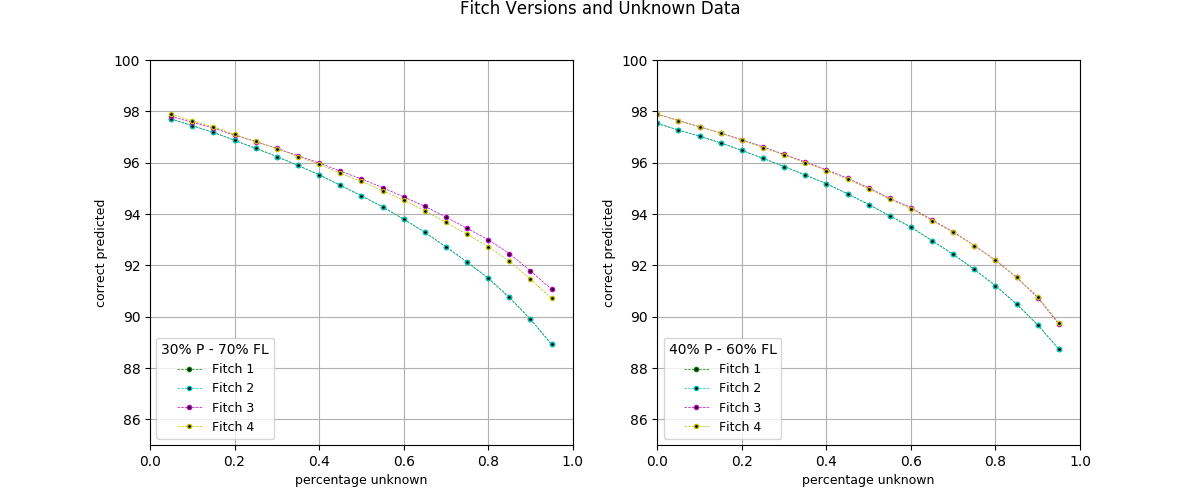
\includegraphics[width=0.6\textwidth]{Figures/simulation_fitch_evaluation.png}
        \end{figure}

        How to extend Fitch for multifunction?:
        \begin{figure}
          \caption{bla}
          \centering
            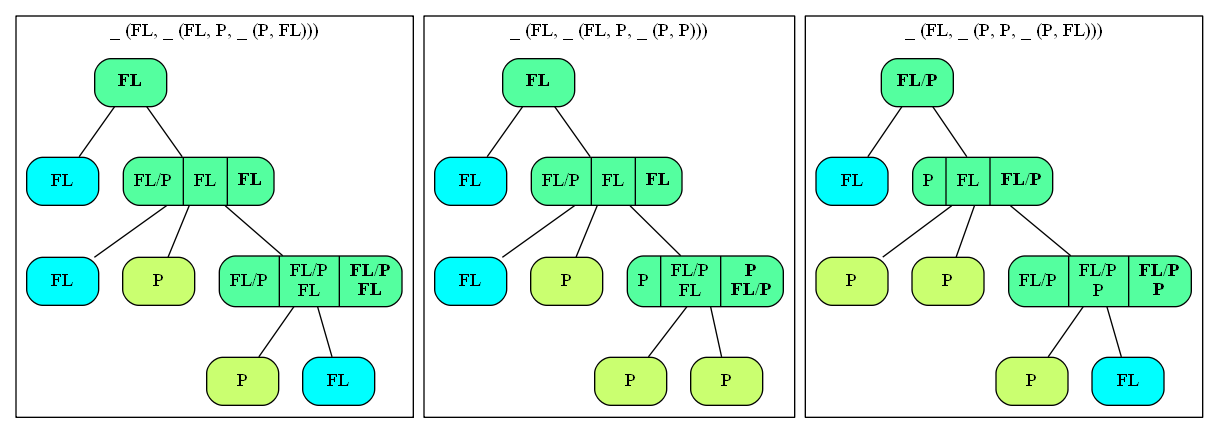
\includegraphics[width=1\textwidth]{Figures/Fitch2.png}
        \end{figure}

      %---------------------------------------------------------------------------------------------------
      \subsubsection{Sankoff}
        Maximum parsimony algorithm from Sankoff implemented in the R package castor \cite{Louca2017}.

      %---------------------------------------------------------------------------------------------------  
      \subsubsection{my Algorithm}

  %---------------------------------------------------------------------------------------------------
  %---------------------------------------------------------------------------------------------------
  %---------------------------------------------------------------------------------------------------
  \section{real data analysis}
    \begin{itemize}
      \item Import tree
      \item Import interactions
      \item run castor algorithm / and others?
      \item interprete results (leave one out)
    \end{itemize}

  %---------------------------------------------------------------------------------------------------
  %---------------------------------------------------------------------------------------------------
  %---------------------------------------------------------------------------------------------------
  \section{Implementation}

%---------------------------------------------------------------------------------------------------
%---------------------------------------------------------------------------------------------------
%---------------------------------------------------------------------------------------------------
%---------------------------------------------------------------------------------------------------
\chapter{Results}
  A big point in this chapter is the result of examining the input data. How is the situation? What 
    influence does that have on our actual result? What can we do about it? Our simulation gave us 
    some results to this. \\
  Otherwise, this chapter is mainly about the actual reconstruction of the states. This means, on 
    one hand investigation of origins and losses of the inner nodes and on the other, the prediction 
    of unknown states of leaf nodes. \\
   
  %---------------------------------------------------------------------------------------------------
  %---------------------------------------------------------------------------------------------------
  %---------------------------------------------------------------------------------------------------
  \section{Metadata analysis}

    %---------------------------------------------------------------------------------------------------
    %---------------------------------------------------------------------------------------------------
    \subsection{Taxa}
      The investigation of the taxonomy revealed that our tree has three kingdoms: Chloroplastida, 
        Metazoa, Fungi, 53 phyla, 195 classes and 924 orders. \\
      Since the analysis of the tree is not part of this work, it should be mentioned here that, 
        according to recent findings, this is not complete and we lack some taxa in every rank. For 
        example, Hans says that one distinguishes between seven and nine kingdoms 
        \cite{CavalierSmith1981}. \\
      In section \pageref{sec:listPhyla} of the appendix you can find a list of all phyla.
      
    %---------------------------------------------------------------------------------------------------
    %---------------------------------------------------------------------------------------------------
    %---------------------------------------------------------------------------------------------------
    \section{Multifurcation}\label{sec:ResultsMultifurcation}
      One property of the tree is its ridge of multifurcation. A complete phylogenetic tree would be 
        binary, which means the number of leaf nodes is closely to the number of internal nodes. But 
        since we only work with a synthesis tree, this tree is multifurcated: we have 241 974 internal 
        nodes and 2 293 463 leaf nodes. \\
      For a first overview we collected for every node its number of children (degree $-1$), and plotted
        this in an histogram, see figure \ref{fig:childrenOfNodes}. The multifurcation affects only the
        internal nodes. We collected the number of children $-2$ of every node (a node with two children 
        is binary). 
      \begin{wrapfigure}{r}{0.6\textwidth}
        \begin{center}
          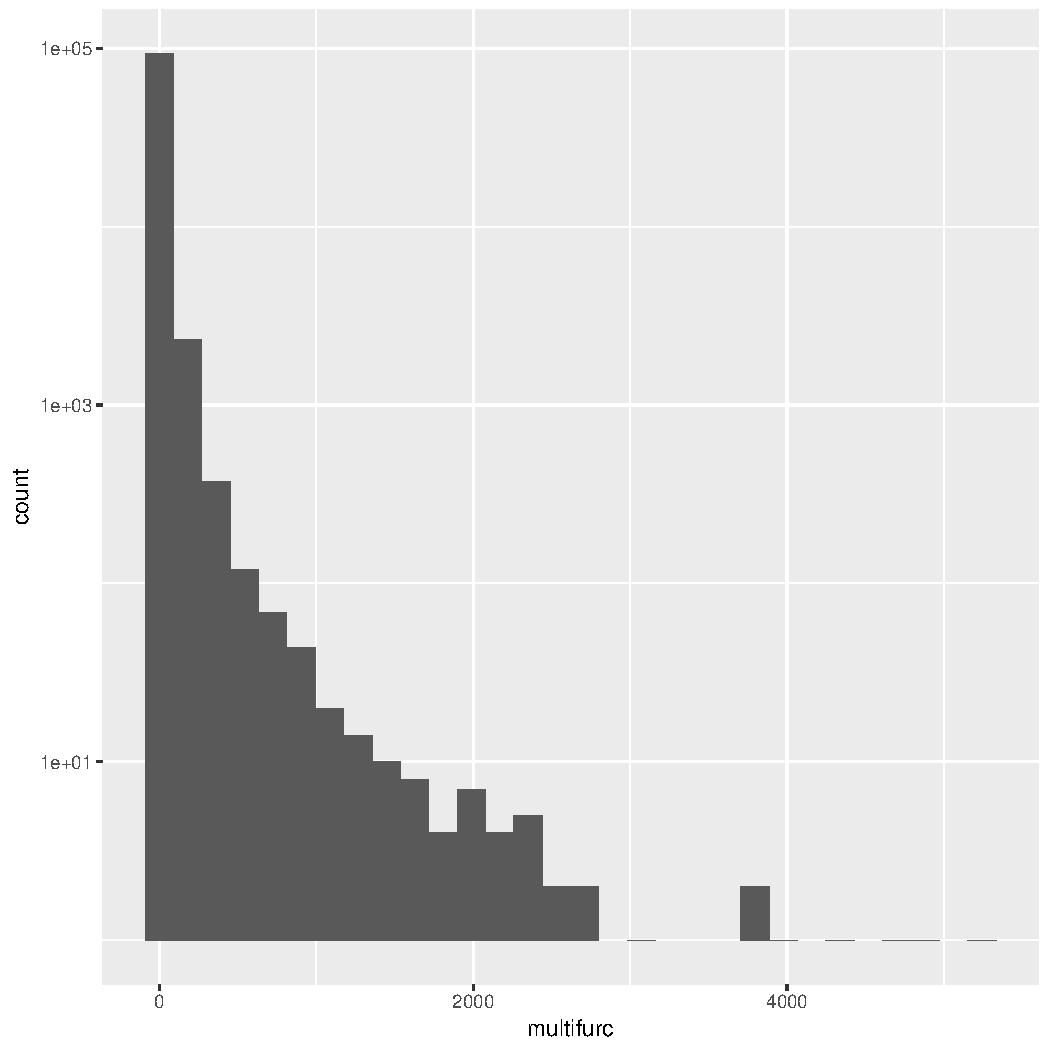
\includegraphics[trim = 0mm 0mm 30mm 0mm, clip, width=0.58\textwidth]{Figures/multifurc.pdf}
        \end{center}
        \caption{Histogram about the multifurcation of the internal nodes of the synthesis tree. \\ 
          light blue: binary; dark blue: multifunction}
        \label{fig:childrenOfNodes}
      \end{wrapfigure}
      That means it discribes the number of nodes which we have lost from the real (binary) 
      phylogenetic tree. \\
      As you can see, we are very far from a binary tree.
    
      %---------------------------------------------------------------------------------------------------
      \subsubsection{Data artifacts}
      At this point we also found out that there are some nodes with only one child node (55700 nodes). \\
      These are both, the most nodes are right in front of a leaf, as well as some nodes are deep in the 
        tree (3956 with height $>2$). They are probably a result from the fact that taxonomic information 
        has been incorporated into a phylogeny. \\
      Some examples:
      \begin{itemize}
        \item Nephroselmidophyceae: (class) \\
          https://tree.opentreeoflife.org/opentree/argus/ottol@1038762
        \item Phrynocrinidae: (family) \\
          https://tree.opentreeoflife.org/opentree/argus/ottol@3647979
        \item Elaeocarpus sylvestris: \\
          https://tree.opentreeoflife.org/opentree/argus/opentree9.1@ott166969
      \end{itemize}
     
      %---------------------------------------------------------------------------------------------------
      %---------------------------------------------------------------------------------------------------
      \subsection{Poisson regression}
        glm (generalized linear model) analysis: \\
      
        
        The intercept is $2.821 > 0$ $\Rightarrow$ there is a multifunction.
        (Intercept: Stärke der Multifurcation) \\
        Comparing the different kingdoms, we find that multifunctionality is greater in Fungi than in 
        Chloroplastida than in Metazoa:
        $$4.0999 (Fungi Intercept) > -0.9132 (Chloroplastida Intercept) > -1.4320 (Metazoa Intercept)$$
        % Degrees of Freedom: 96010 Total (i.e. Null);  96010 Residual
        Wir haben außerdem drei komplexitätsstärken von Modellen verglichen bezüglich der höhe und tiefe 
          des Baums mit dem folgenden Deviance Table:
          
        \begin{table}[h]
          \begin{center}
            \begin{tabular}{ |l|r|r|r|r| }
              \hline
              Model / Taxa & Kingdom & Phylum & Class & Order \\
              \hline \hline
              multifurc $\sim$ taxa & 7774454 & 7435700 & 7337241 & 7076068 \\
              \hline
              multifurc $\sim$ taxa + depth & 7752303 & 7431609 & 7334754 & 7027578 \\
              multifurc $\sim$ taxa + max.height & 7730196 & 7375889 & 7275856 & 7005424 \\
              multifurc $\sim$ taxa + min.height & 7472500 & 7233486 & 7144686 & \cellcolor{green!50}6890703 \\
              multifurc $\sim$ taxa + mean.height & 7304402 & 7128318 & 7055313 & \cellcolor{green!50}6815271 \\
              \hline
              multifurc $\sim$ taxa * depth & 7714881 & 7335396 & 7250759 & \cellcolor{green!50}6843004 \\
              multifurc $\sim$ taxa * max.height & 7692980 & 7311241 & 7187504 & \cellcolor{green!50}6795823 \\
              multifurc $\sim$ taxa * min.height & 7442387 & 7177002 & 7094933 & \cellcolor{green!50}6795099 \\
              multifurc $\sim$ taxa * mean.height & 7247309 & 7020258 & \cellcolor{green!50}6965794 & \cellcolor{green!50}6665565 \\
              \hline
            \end{tabular} 
          \end{center}
          \caption{Residuals...}
          \label{table:...} 
        \end{table}
        * Residuals: Fehler - wieviele Werte sind nicht gut modelliert. (umso kleiner umso besser - grün) \\

        \begin{lstlisting}[gobble=8]
          class * depth / min/max/mean.height: Warning message: glm.fit: fitted rates numerically 0 occurred
          order * depth / min/max/mean.height: Error: cannot allocate vector of size 2.2 Gb
        \end{lstlisting}

        Interpretation: Die Multifurkation ist sehr ungleich verteilt. Daher ist die vorhersage umso 
          genauer umso kleinere Subtrees wir betrachten. ...
        
        \anmerkung{different parameters for different taxa? (Emanuel)} \\ \\

        Because of the difference in the complexity of the models, we compared their BICs:
        \begin{table}[h]
          \begin{center}
            \begin{tabular}{ |l|r|r|r|r| }
              \hline
              Model / Taxa & Kingdom & Phylum & Class & Order \\
              \hline \hline
              multifurc $\sim$ taxa & 8273333 & 7937828 & 7842157 & 7644249\\
              \hline
              multifurc $\sim$ taxa + depth & 8273318 & 7934322 & 7839364 & \cellcolor{green!50}7539999 \\
              multifurc $\sim$ taxa + max.height & 7993515 & 7749121 & 7661817 & \cellcolor{green!50}7416211 \\
              multifurc $\sim$ taxa + min.height & 8251211 & 7875521  & 7778327 & \cellcolor{green!50}7516883 \\
              multifurc $\sim$ taxa + mean.height & 7825417 & 7644249 & \cellcolor{green!50}7572474 & \cellcolor{green!50}7340741 \\
              \hline
              multifurc $\sim$ taxa * depth & 8235932 & 7836755 & 7757688 & \cellcolor{green!50}7383808 \\
              multifurc $\sim$ taxa * max.height & 7963438 & 7693555 & 7614820 & \cellcolor{green!50}7335338 \\
              multifurc $\sim$ taxa * min.height & 8214030 & 7808940 & 7690618 & \cellcolor{green!50}7336627\\
              multifurc $\sim$ taxa * mean.height & 7768360 & \cellcolor{green!50}7536296 & \cellcolor{green!50}7484953 & \cellcolor{green!50}7206369 \\
              \hline
            \end{tabular} 
          \end{center}
          \caption{BIC...}
          \label{table:...} 
        \end{table}

  %---------------------------------------------------------------------------------------------------
  %---------------------------------------------------------------------------------------------------
  %---------------------------------------------------------------------------------------------------
  \section{Unknown leaf nodes}
    Next to the problem of the multifurcation of the tree is the less of data we have for the species.
      For the ancestral state reconstruction, we need information in the leaf nodes. \\
    The eukaryotic synthesis tree has 293 463 leaf nodes. The GloBI database has 5 346 414 interactions 
      (at this timepoint). Out of this data we got 51 337 distinct free-living species and 47 332 
      distinct parasite species $\rightarrow$ unknown nodes 2194794 ($\approx 95.7\%$). \\
    With this only $\approx 4.3\%$ information in our leaf nodes are 

    \todo{einbauen?:} \\
    unused possible species  57 352 (source), \\
    809 993 (target) \\
    \#interactions zu \#Parasiten und \#Freilebend $\rightarrow$ Wieviel gibt GloBI her? (dazu noch 
      \#unused possible species, wieviele Parasiten ohne ott haben wir gefunden?)

    %---------------------------------------------------------------------------------------------------
    %---------------------------------------------------------------------------------------------------
    \subsection{Results of simulation / Influence of different parameters}

    \begin{figure}
      \caption{Influence of unknown data to prediction}
      \centering
      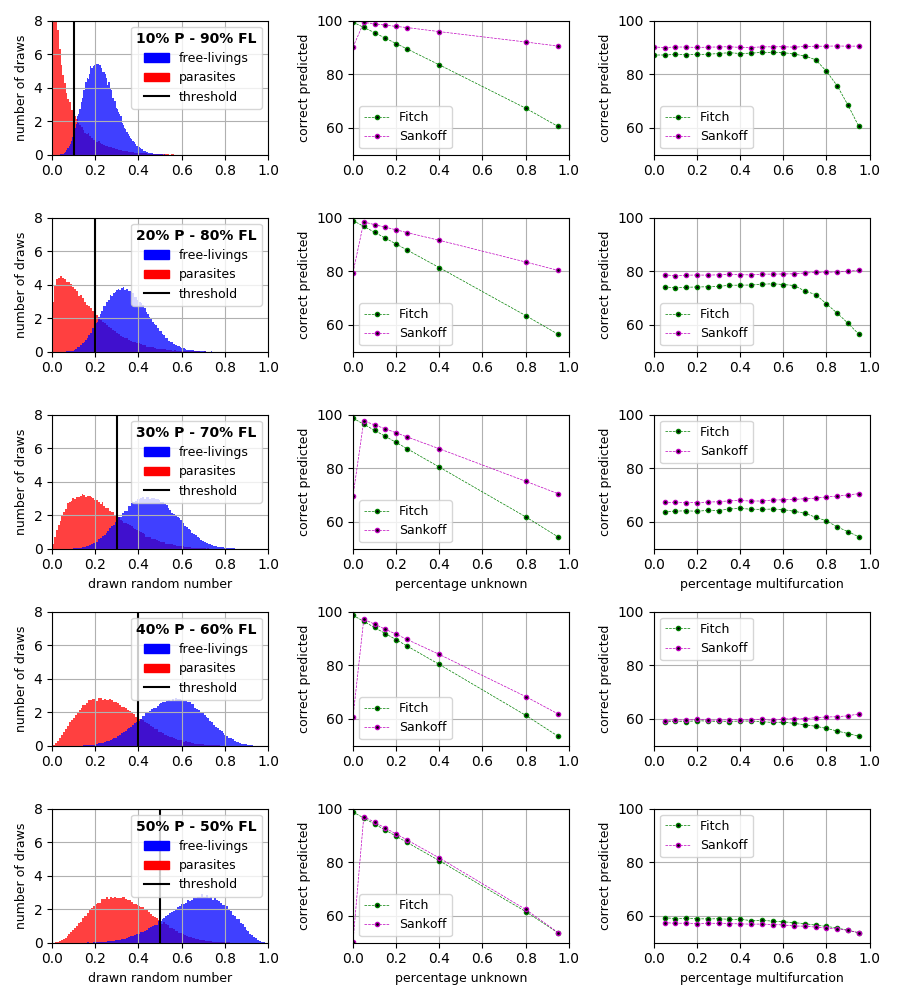
\includegraphics[trim = 0mm 0mm 0mm 50mm, clip,width=0.9\textwidth]{Figures/simulation_evaluation_1.png}
    \end{figure}

  %---------------------------------------------------------------------------------------------------
  %---------------------------------------------------------------------------------------------------
  %---------------------------------------------------------------------------------------------------
  \section{Results of castor}

    %---------------------------------------------------------------------------------------------------
    %---------------------------------------------------------------------------------------------------
    \subsection{Biological view}
    

      \todo{Castor replaces originaltags with finaltags. There are 82 originaltags != finaltag.} \\ \\

      We picked a few phyla to evaluate the results from the biological point of view. \\
      Table \ref{table:phylum leaf nodes states} shows some known phyla: Chordata, Nematoda, 
        Platyhelminthes and Apicomplexa. \\
      As we know \todo{ref einfügen} the Chordata are full of free-living species and there are only a 
        few parasites. The algorithm reflects this. We started with 99.83\% free-living species and 
        predicted 99.94\% species as parasites \todo{(inklusive all known nodes)}. Only 0.06\% were 
        predicted as parasites. These few parasites are mostly breeding parasites (brood parasitism) and 
        some individual errors from the GloBI database. \\
      Same observation but with less free-livings is the Apicomplexa Phylum. Here we have only a few 
        free-livings \todo{ref einfügen}. And as we see, we had good start data and predicted 00.95\% as 
        parasites. \\
      For the Platyhelminthes the literature says that there are mostly all Platyhelminthes parasites
        \todo{ref einfügen}. But at the end we predicted 4.18\% as free-living. The class Seriata is the 
        reason for the most of free-livings in this phylum. These are partly free-living flatworms, so 
        the prediction looks right. \\
        \todotext{ Wiki: \\
        *The Seriata are an order of turbellarian flatworms.[1][2] \\
        They are found in both freshwater and marine environments, and also include a number of species 
        found in damp terrestrial conditions. Most are free-living, but the group includes the genus 
        Bdelloura, which lives comensally on the gills of horseshoe crabs. Seriatans are distinguished 
        from other related groups by the presence of a folded pharynx and of a number of diverticula 
        arising from the intestine. The intestine itself may be either simple or branched.[3]}
      
      With the Nematoda it looks very different.  In the Nematoda its much worse. Here speaks the 
        literature of \todo{x percent} free-living, but we found only 2.63\% of them. The problem at 
        this point, however, is obvious: The parasites have been much more studied and thus we start 
        with only 0.63\% free-living species. Against such a shifted data situation, the algorithm is 
        powerless. And yet the percentage has increased.

      \begin{table}
        \begin{center}
          \hspace*{-1cm}\begin{tabular}{ |l|r||r|r||r|r|r|r|r|r| }
            \hline
            & & \multicolumn{2}{c||}{original states} & \multicolumn{6}{c|}{final states} \\
            Phylum & \# nodes & FL & P
              & 0 (FL) & 0.4 & 0.5 & 0.67 & 0.75 & 1 (P) \\
            \hline \hline
            Chordata & 91785 & 10451 & 18 
              & 91734 & 0 & 0 & 0 & 0 & 51 \\
            & & 99.83\% & 0.49\%
              & 99.94\% & & & & & 0.06\% \\ \hline
            Nematoda & 30127 & 21 & 3289 
              & 791 & 0 & 1017 & 0 & 0 & 28319 \\
            & & 0.63\% & 99.37\%
              & 2.63\% & & 3.38\% & & & 94\% \\ \hline
            Platyhelminthes & 22683 & 7 & 7086 
              & 949 & 0 & 151 & 0 & 0 & 21583 \\
            & & 0.1\% & 99.9\%
              & 4.18\% & & 0.67\% & & & 95.15\% \\ \hline
            Apicomplexa & 1863 & 1 & 255 
              & 1 & 0 & 0 & 0 & 0 & 1862 \\
            & & 0.39\% & 99.61\%
              & 0.05\% & & & & & 99.95\% \\
            \hline \hline
            Arthropoda & 1198981 & 18912 & 11141 
              & 1099509 & 1313 & 22478 & 4176 & 1665 & 70223 \\
            & & 62.93\% & 37.07\%
              & 91.7\% & 0.11\% & 1.87\% & 0.35\% & 0.14\% & 5.86\% \\
            \hline
          \end{tabular} 
        \end{center}
        \caption{Phylum (leaf nodes)}
        \label{table:phylum leaf nodes states} 
      \end{table}

      \anmerkungstext{Das sind schonmal vier große Kontraste, wenn dann noch Zeit bleibt, die 
        schwirigen... Arthropoden, Fungi, Pflanzen... (Emanuel)} \\

      \begin{table}
        \begin{center}
          \hspace*{-2cm}\begin{tabular}{ |l|r||r|r||r|r|r|r|r|r|r|r| }
            \hline
            & & \multicolumn{2}{c||}{original states} & \multicolumn{8}{c|}{final states} \\
            Kingdom & \# nodes & FL & P
              & 0 (FL) & 0.25 & 0.33 & 0.4 & 0.5 & 0.67 & 0.75 & 1 (P) \\
            \hline \hline
            none & 84456 & 45 & 529 
              & 15035 & 243 & 25910 & 0 & 8764 & 6183 & 0 & 28140 \\
            Fungi & 324105 & 577 & 2983
              & 39088 & 0 & 0 & 0 & 5858 & 0 & 0 & 274803 \\
            Chloroplastida & 460457 & 3519 & 77
              & 454211 & 0 & 0 & 0 & 4688 & 0 & 0 & 1558 \\
            Metazoa & 1670956 & 30758 & 22373
              & 1485749 & 0 & 0 & 1313 & 29002 & 5102 & 1957 & 147833 \\
            \hline  
          \end{tabular}
        \end{center}
        \caption{Kingdom (inkl internal nodes)}
      \end{table}

      \begin{table}
        \begin{center}
          \begin{tabular}{ |l|r||r|r||r|r|r|r|r|r| }
            \hline
            & & \multicolumn{2}{c||}{original states} & \multicolumn{6}{c|}{final states} \\
            Phylum & \# nodes & FL & P
              & 0 (FL) & 0.4 & 0.5 & 0.67 & 0.75 & 1 (P) \\
            \hline \hline
            Chordata & 122546 & 10451 & 18 
              & 122473 & 0 & 0 & 0 & 0 & 73 \\
            Nematoda & 33564 & 21 & 3289 
              & 846 & 0 & 1133 & 0 & 0 & 31585 \\
            Platyhelminthes & 27142 & 7 & 7086 
              & 1010 & 0 & 175 & 0 & 0 & 25957 \\
            Apicomplexa & 2102 & 1 & 255 
              & 1 & 0 & 0 & 0 & 0 & 2101 \\
            \hline
            Arthropoda & 1319460 & 18912 & 11141 
              & 1207204 & 1313 & 25499 & 4852 & 1957 & 78635 \\
            \hline
          \end{tabular}
        \end{center}
        \caption{Phylum (inkl internal nodes)}
      \end{table}

      \begin{table}
        \begin{center}
          \hspace*{-2cm}\begin{tabular}{ |l|r||r|r||r|r|r|r|r|r|r|r| }
            \hline
            & & \multicolumn{2}{c||}{original states} & \multicolumn{8}{c|}{final states} \\
            Kingdom & \# nodes & FL & P
              & 0 (FL) & 0.25 & 0.33 & 0.4 & 0.5 & 0.67 & 0.75 & 1 (P) \\
            \hline \hline
            none & 75446 & 45 & 529 
              & 13426 & 220 & 24082 & 0 & 7792 & 5302 & 0 & 24493 \\
            Fungi & 31457 & 577 & 2983
              & 38520 & 0 & 0 & 0 & 5723 & 0 & 0 & 266463 \\
            Chloroplastida & 416478 & 3519 & 77
              & 410795 & 0 & 0 & 0 & 4182 & 0 & 0 & 1501 \\
            Metazoa & 1491012 & 30758 & 22373
              & 1328135 & 0 & 0 & 930 & 25535 & 4423 & 1665 & 130324 \\
            \hline  
          \end{tabular}
        \end{center}
        \caption{Kingdom (leaf nodes)}
      \end{table}

\newpage
    %---------------------------------------------------------------------------------------------------
    %---------------------------------------------------------------------------------------------------
    \subsection{Origins and Losses}

      Sara B. Weinstein and Armand M. Kuris have been searching for origins of parasitism in Animalia 
        \cite{Weinstein2016}. They identified 223 parasitic origins: 223 in Metazoa $\supset$ 143 in 
        Arthropoda $\supset$ 87 in Insecta. \\
      This has led us to count the origins and losses of parasitism in our investigation as well. \\
      We count only one origin / loss in a parent node with different children's nodes. \\
      Here we have encountered a problem: The Castor algorithm gives us probabilities for states. That 
        means there are also nodes with state like 0.3 or 0.5. So how do you count? Our solution was, 
        to round these values. We have to say that we round 0.5 to 0.

      \begin{table} [h]
        \begin{center}
          \begin{tabular}{ |l|r|r||r|r|r| }
            \hline
            Domain  & \# internal & \# leaf & Rootnode & \multicolumn{2}{c|}{without and with rounding} \\ 
            / Kingdom  & \multicolumn{2}{c||}{nodes} & state & \# origins & \# losses \\
            / Phylum / Class & & & & (FL -> P) & (P -> FL) \\
            \hline \hline
            Eukaryota & 241974 & 2293463 & 1.0 & 415 & 363 \\
            & & & P & 462 & 369 \\
            \hline \hline
            Metazoa & 179944 & 1491012 & 0.5 & 294 & 123 \\
            & & & & 321 & 129 \\ \hline
            Fungi & 9534 & 314571 & 0.5 & 80 & 222 \\
            & & & & 97 & 222 \\ \hline
            Chloroplastida & 43486 & 412434 & 0.0 & 40 & 2 \\
            & & & FL & 42 & 2 \\
            \hline \hline            
            Arthropoda & 120479 & 1198981 & 0.0 & 260 & 102 \\
            & & & FL & 281 & 108 \\ \hline
            Apicomplexa & 239 & 1863 & 1.0 & 0 & 1 \\
            & & & P & 0 & 1 \\ \hline
            Nematoda & 3437 & 30127 & 1.0 & 0 & 11 \\
            & & & P & 2 & 11 \\ \hline
            Chordata & 30761 & 91785 & 0.0 & 12 & 1 \\
            & & & FL & 12 & 1 \\ \hline
            Platyhelminthes & 4459 & 22683 & 1.0 & 0 & 5 \\
            & & & P & 0 & 5 \\
            \hline \hline            
            Insecta & 91256 & 989572 & 0.0 & 234 & 77 \\
            & & & FL & 245 & 77 \\ 
            \hline  
          \end{tabular}
        \end{center}
        \caption{Origins and losses}
        \label{table:origins and losses} 
      \end{table}

      In Table \ref{table:origins and losses} we can see, that we found some more origins than Weinstein 
        and on top of that some losses. \\
      
      Lets have a look at the same phyla as in the section before: Chordata, Nematoda, 
        Platyhelminthes and Apicomplexa. \\
      Chordata are full of free-living species and so we see only a few origins of parasitism. The root
      and mostly all species are predicted as free-living. \\
      In Apicomplexa and the Platyhelminthes are looking fine too. Our algorithm gives us only one loss 
        of parasitism in Apicomplexa and five in the Platyhelminthes. They are both from the root over 
        mostly all species predicted as parasites. \\
      Nematoda is again full of problems. The rootnode is predicted as a parasite and so we have more 
        losses of parasitism for the less information of free-living species in this phylum. The rest 
        is parasitic \\

      \begin{lstlisting}[gobble=6]
        # possible tags: 0, 0.333, 0.4, 0.5, 0.667, 0.75, 1
        # rounded to:    0  0      0    0    1      1     1
        if node_state != father_state:
          if father_state == 0:
              origins += 1        # FL -> P
              new_found = True
          else:
              losses += 1         # P -> FL
              new_found = True
      \end{lstlisting}

      \todo{without rounding change else: to elif $father_state == 1$}
      
    %---------------------------------------------------------------------------------------------------
    %---------------------------------------------------------------------------------------------------
    \subsection{Cross evaluation - leave 100 out}
      We ran the castor algorithm (\todo{10000}) 10 times with leaving 100 randomized free-living or 
        parasitic species out of the input data to see how stable our result is. \\
      What could happen by removing a parasite or free-living of the list?
      \begin{itemize}
        \item It could be a specie, which don't exist in the tree leaf nodes. -> no effect
        \item It could be a specie, which exists in both lists. -> If it was a parasite, it is now 
          free-living, because we prefer parasites. Otherwise we have no effect again. (1053 are possible)
        \item Normal case: We loose information, because its a specie in our tree and we change it to a 
          leave node with no information.
      \end{itemize}
      \begin{table}
        \begin{center}
          \begin{tabular}{ |c||r|r|r||c|r| }
            \hline
            run & \multicolumn{3}{c||}{distance} & changed & lost \\
            & all nodes & leaf nodes & internal nodes & tag & tag \\
            \hline \hline
            0 & 4.0 & 4.0 & 0.0 & 4 & 48 \\
            1 & 4.0 & 4.0 & 0.0 & 2 & \cellcolor{green!50}45 \\
            2 & 85.3 & 79.3 & 6.0 & 3 & 51 \\
            3 & 1.0 & 1.0 & 0.0 & 1 & 47 \\
            \rowcolor{red!50}4 & 1248.0 & 1230.5 & 17.5 & \cellcolor{green!50}0 & 54 \\
            5 & 169.0 & 168.0 & 1.0 & 3 & 52 \\
            6 & 1.0 & 1.0 & 0.0 & 1 & 48 \\
            7 & 1.0 & 1.0 & 0.0 & 1 & 53 \\
            8 & 1.0 & 1.0 & 0.0 & 1 & \cellcolor{red!50}54 \\
            9 & 1.0 & 1.0 & 0.0 & 1 & 52 \\
            \hline
          \end{tabular}
        \end{center}
        \caption{Example runs. \\ green: min value, red: max value}
      \end{table}

      \begin{table}
        \begin{center}
          \begin{tabular}{ |cl||r|r|r|r| }
            \hline
            & & min & max & mean & variance \\
            \hline \hline
            \multirow{3}{*}{distance} & all & 1.0 & 1248.0 & 151.53 & 151528.92 \\
            & leaf nodes                    & 1.0 & 1230.5 & 149.08 & 147380.74 \\
            & internal nodes                & 0.0 & 17.5 & 2.45 & 31.47 \\ \hline
            \multicolumn{2}{|c||}{changed tag} & 0.0 & 4.0 & 1.7 & 1.57 \\ \hline
            lost tag & all tags             & 45.0 & 54.0 & \cellcolor{green!50}50.40 & 10.04 \\
            & FL tags                       & 16.0 & 32.0 & 23.10 & 18.77 \\
            & P tags                        & 16.0 & 36.0 & 27.30 & 41.34 \\
            \hline
          \end{tabular}
        \end{center}
        \caption{Statistics to Cross validation}
      \end{table}
  
%---------------------------------------------------------------------------------------------------
%---------------------------------------------------------------------------------------------------
%---------------------------------------------------------------------------------------------------
%---------------------------------------------------------------------------------------------------
\chapter{Discussion}
  Wie gut ist der randomisiert erstellte Baum? \\
  Wie gut kommt unsere Simulation an die echte Datenlage heran. \\
  Fehlerqoute der Daten an sich? \\
  Wie gut ist unsere Datenlage? 3 mio knoten, 1.8 named species (leaf nodes), 200.000 leaf nodes mit 
  Information. \\
  Simulation von subtrees \\
  Welche Teile des Baumes sind gut, an welchen muss noch viel geforscht werden. \\
  Wieviele Origins haben wir gefunden, was bedeutet diese Zahl? \\
  
  Parameter der Simulation:
  \begin{itemize}
    \item Wie ist die Verteilung der vergessenen internen Knoten? Zum Wurzelknoten hin mehr vergessen?
    \item Wie sehen die übergangswahrscheinlichkeiten aus von P$\rightarrow$FL und andersherum?
    \item Verteilung Parasiten zu Freilebend zu keine Information
  \end{itemize}


  Selecting of the 'right'  / best Distribution
  
%---------------------------------------------------------------------------------------------------
%---------------------------------------------------------------------------------------------------
%---------------------------------------------------------------------------------------------------
\bibliography{bibliographie}

%---------------------------------------------------------------------------------------------------
%---------------------------------------------------------------------------------------------------
%---------------------------------------------------------------------------------------------------
\chapter{Appendices}
  %---------------------------------------------------------------------------------------------------
  %---------------------------------------------------------------------------------------------------
  \section{List of all phyla}\label{sec:listPhyla}

  Phyla (53): \\
  Acanthocephala, Amoebozoa, Apicomplexa, Arthropoda, Ascomycota, Bacillariophyta, Basidiomycota, 
    Brachiopoda, Bryozoa, Chaetognatha, Chlorophyta, Chordata, Chromerida, Chytridiomycota, 
    Ciliophora, Cnidaria, Colponemidia, Ctenophora, Cycliophora, Echinodermata, Entoprocta, 
    Entorrhizomycota, Euglenida, Foraminifera, Gastrotricha, Glomeromycota, Gnathostomulida, 
    Haplosporida, Haptophyta, Hemichordata, Kinorhyncha, Loricifera, Microsporidia, Mollusca, 
    Myzostomida, Nematoda, Nematomorpha, Nemertea, Onychophora, Orthonectida, Phaeophyceae, 
    Picozoa, Placozoa, Platyhelminthes, Porifera, Priapulida, Rhodophyta, Rhombozoa, Rotifera, 
    Streptophyta, Tardigrada, Xanthophyceae \\
  Wobei von Streptophyta -> Anthocerotophyta, Marchantiophyta, Bryophyta, Tracheophyta als
    Phylum im Phylum gefunden und nicht einbezogen wurden und Magnoliophyta als Phylum in 
    Tracheophyta ebenfalls nicht. \\

  %---------------------------------------------------------------------------------------------------
  %---------------------------------------------------------------------------------------------------
  \section{Distribution of data in the taxa}\label{sec:taxaTable1}
    \begin{center}
      \begin{tabular}{ |l|r|l|r|r| }
        \hline
        Kingdom (3) & Number of Nodes & Phylum (25) & Number of Nodes & max max height \\
        \hline \hline
        Metazoa & 1 465 207 & Arthropoda & 1 170 539 & 54 \\
        & & Chordata & 106 650 & 74 \\
        & & Mollusca & 80 022 & 22 \\
        & & Platyhelminthes & 27 141 & 9 \\
        & & Nematoda & 24 564 & 23 \\
        & & Cnidaria & 14 878 & 36 \\
        & & Porifera & 11 737 & 26 \\
        & & Echinodermata & 10 654 & 14 \\
        & & Bryozoa & 8 631 & 11 \\
        & & Rotifera & 3 093 & 7 \\
        & & Nemertea & 1 793 & 7 \\
        & & Tardigrada & 1 654 & 7 \\
        & & Acanthocephala & 1 596 & 6 \\
        & & Brachiopoda & 1 055 & 9 \\
        & & Nematomorpha & 633 & 7 \\
        & & Chaetognatha & 360 & 7 \\
        & & Hemichordata & 196 & 5 \\ 
        & & Cycliophora & 11 & 5 \\ 
        % 1465207-(1170539+106650+80022+27141+24564+14878+11737+10654+8631+3093+1793+1654+1596+1055+633+360+196+11) = 0          \hline
        Fungi & 254 871 & Ascomycota & 157 045 & 19 \\ 
        & & Basidiomycota & 92 931 & 18 \\
        & & Microsporidia & 1 949 & 6 \\ 
        & & Glomeromycota & 1 490 & 6 \\
        & & Chytridiomycota & 1 456 & 6 \\
        % 254871-157045-92931-1949-1490-1456 = 0
        \hline
        Chloroplastida & 121 239 & Streptophyta & 120 731 & 49 \\
        & & Chlorophyta & 508 & 6 \\
        % 121239-120731-508 = 0
        \hline  
      \end{tabular}
    \end{center}

  %---------------------------------------------------------------------------------------------------
  %---------------------------------------------------------------------------------------------------
  \section{Taxa table}\label{sec:taxaTable2}
    \begin{center}
      % \begin{tabular}{ |>{\rowmac}l|>{\rowmac}r|<{\clearrow} }
      \begin{tabular}{ |l|r||r|r|r| }
        \hline
        Taxa & Number of Nodes & Internal Nodes & Leaf Nodes & Terminal Leaf Nodes \\
        \hline \hline
        \setrow{\bfseries}domain & 1 & 1 & &  \\ \hline
        \setrow{\bfseries}kingdom & 3 & 3 & &  \\
        subkingdom & 2 & 2 & & \\
        infrakingdom & 5 & 5 & & \\
        superphylum & 2 & 2 & & \\ \hline
        \setrow{\bfseries}phylum & 57 & 54 & 3 & \\
        subphylum & 22 & 20 & 2 & \\
        infraphylum & 2 & 2 & & \\
        superclass & 8 & 8 & & \\ \hline
        \setrow{\bfseries}class & 209 & 175 & 34 & \\
        subclass & 120 & 106 & 14 & \\
        infraclass & 14 & 11 & 3 & \\
        superorder & 40 & 37 & 3 & \\ \hline
        \setrow{\bfseries}order & 1014 & 772 & 242 & \\
        suborder & 285 & 222 & 63 & \\
        infraorder & 95 & 78 & 17 & \\
        parvorder & 14 & 12 & 2 & \\
        superfamily & 829 & 626 & 203 & \\ \hline
        \setrow{\bfseries}family & 8449 & 6143 & 2306 & \\
        subfamily & 3090 & 2250 & 840 & \\
        supertribe & 1 & 0 & 1 & \\
        tribe & 1764 & 1285 & 479 & \\
        subtribe & 435 & 359 & 77 & \\ \hline
        \setrow{\bfseries}genus & 164656 & 105452 & 59204 & \\
        subgenus & 1266 & 869 & 397 & \\
        section & 3 & 2 & 1 & \\
        subsection & 1 & 1 & 0 & \\
        species group & 365 & 288 & 77 & \\
        species subgroup & 123 & 100 & 23 & \\ \hline
        \setrow{\bfseries}species & 2247251 & 7423 & 2239828 & 2228993 \\
        subspecies & 22437 & 75 & 22362 & 22239 \\
        variety & 1755 & 7 & 1748 & 1726 \\
        varietas & 5970 & 19 & 5951 & 5909 \\
        forma & 1181 & & 1181 & 1181 \\
        \hline \hline
        no rank & 954 & 719 & 235 & 7 \\
        no rank - terminal & 37452 & & 37452 & 37452 \\
        (no entry) & 40099 & 40099 & & \\
        \hline  
      \end{tabular}
    \end{center}
    extended leaf nodes (real leaf nodes)

\end{document}
